% Claude Code Knowledge Architecture — Beamer Presentation
% Building Persistent Intelligence for AI-Assisted Research
\documentclass[aspectratio=169,11pt]{beamer}

\usetheme{Madrid}
\usepackage{tikz}
\usetikzlibrary{shapes.geometric, arrows.meta, positioning, calc, fit, backgrounds, decorations.pathreplacing}
\usepackage{listings}
\usepackage{fancyvrb}
\usepackage{xcolor}
\usepackage{hyperref}
\usepackage{array}
\usepackage{booktabs}

% ── Color palette ──────────────────────────────────────────────
\definecolor{cPrimary}{HTML}{2D3748}      % dark slate
\definecolor{cAccent}{HTML}{3182CE}       % blue
\definecolor{cAccentDark}{HTML}{2B6CB0}   % darker blue
\definecolor{cGreen}{HTML}{38A169}        % green
\definecolor{cOrange}{HTML}{DD6B20}       % orange
\definecolor{cRed}{HTML}{E53E3E}         % red
\definecolor{cPurple}{HTML}{805AD5}       % purple
\definecolor{cGray}{HTML}{718096}         % gray
\definecolor{cLightBg}{HTML}{EBF4FF}      % light blue bg
\definecolor{cLightGreen}{HTML}{F0FFF4}   % light green bg
\definecolor{cLightOrange}{HTML}{FFFAF0}  % light orange bg
\definecolor{cCodeBg}{HTML}{F7FAFC}       % code background

% ── Theme customization ───────────────────────────────────────
\setbeamercolor{palette primary}{bg=cPrimary,fg=white}
\setbeamercolor{palette secondary}{bg=cAccent,fg=white}
\setbeamercolor{palette tertiary}{bg=cAccentDark,fg=white}
\setbeamercolor{palette quaternary}{bg=cPrimary,fg=white}
\setbeamercolor{structure}{fg=cAccent}
\setbeamercolor{title}{fg=white,bg=cPrimary}
\setbeamercolor{frametitle}{fg=white,bg=cPrimary}
\setbeamercolor{block title}{bg=cAccent,fg=white}
\setbeamercolor{block body}{bg=cLightBg,fg=cPrimary}
\setbeamercolor{block title alerted}{bg=cOrange,fg=white}
\setbeamercolor{block body alerted}{bg=cLightOrange,fg=cPrimary}
\setbeamercolor{block title example}{bg=cGreen,fg=white}
\setbeamercolor{block body example}{bg=cLightGreen,fg=cPrimary}
\setbeamercolor{item}{fg=cAccent}
\setbeamercolor{subitem}{fg=cGray}
\setbeamercolor{footnote}{fg=cGray}

\setbeamertemplate{navigation symbols}{}
\setbeamertemplate{footline}{%
  \leavevmode%
  \hbox{%
    \begin{beamercolorbox}[wd=.33\paperwidth,ht=2.25ex,dp=1ex,center]{palette primary}%
      \usebeamerfont{author in head/foot}\insertshortauthor
    \end{beamercolorbox}%
    \begin{beamercolorbox}[wd=.34\paperwidth,ht=2.25ex,dp=1ex,center]{palette secondary}%
      \usebeamerfont{title in head/foot}\insertshorttitle
    \end{beamercolorbox}%
    \begin{beamercolorbox}[wd=.33\paperwidth,ht=2.25ex,dp=1ex,right]{palette primary}%
      \insertframenumber{} / \inserttotalframenumber\hspace*{2ex}
    \end{beamercolorbox}}%
  \vskip0pt%
}

% ── Listings config ───────────────────────────────────────────
\lstset{
  basicstyle=\ttfamily\scriptsize,
  backgroundcolor=\color{cCodeBg},
  frame=single,
  rulecolor=\color{cGray!40},
  keywordstyle=\color{cAccent}\bfseries,
  commentstyle=\color{cGray}\itshape,
  stringstyle=\color{cGreen},
  breaklines=true,
  columns=fullflexible,
  keepspaces=true,
  showstringspaces=false,
  xleftmargin=4pt,
  xrightmargin=4pt,
  aboveskip=6pt,
  belowskip=4pt,
}

% ── TikZ styles ───────────────────────────────────────────────
\tikzset{
  layerbox/.style={
    draw=#1, fill=#1!8, rounded corners=4pt,
    minimum width=12cm, minimum height=1.5cm,
    font=\small, text=cPrimary, line width=1pt,
    inner sep=8pt,
  },
  smallbox/.style={
    draw=#1, fill=#1!10, rounded corners=3pt,
    minimum width=2.8cm, minimum height=0.9cm,
    font=\footnotesize, text=cPrimary, line width=0.8pt,
    align=center,
  },
  flownode/.style={
    draw=cAccent, fill=cAccent!10, rounded corners=3pt,
    minimum width=2.2cm, minimum height=0.8cm,
    font=\footnotesize, text=cPrimary, line width=0.8pt,
    align=center,
  },
  decisionnode/.style={
    draw=cOrange, fill=cOrange!10, diamond,
    minimum width=1.8cm, minimum height=1cm,
    font=\footnotesize, text=cPrimary, line width=0.8pt,
    align=center, aspect=1.8,
  },
  arw/.style={-{Stealth[length=5pt]}, thick, color=#1},
  arw/.default=cAccent,
  brace/.style={decorate, decoration={brace, amplitude=6pt, raise=2pt}},
}

% ── Meta ──────────────────────────────────────────────────────
\title[Knowledge Architecture]{Building Persistent Intelligence\\for AI-Assisted Research}
\subtitle{A Knowledge Architecture for Claude Code}
\author[L.\ Santucci]{Larry Santucci}
\institute{Federal Reserve Bank of Philadelphia}
\date{\today}

\begin{document}

% ══════════════════════════════════════════════════════════════
% TITLE
% ══════════════════════════════════════════════════════════════
\begin{frame}[plain]
\titlepage
\vspace{-6pt}
{\centering\scriptsize\color{cGray}%
The views expressed herein are solely those of the author and do not necessarily reflect the views of the Federal Reserve Bank of Philadelphia or the Federal Reserve System. Nothing in the text should be construed as an endorsement of any organization or its products or services. This presentation is a co-creation of the author and Claude Code for VS Code version 2.1.72.\par}
\end{frame}

% ══════════════════════════════════════════════════════════════
% THE PROBLEM
% ══════════════════════════════════════════════════════════════
\begin{frame}[shrink=5]{The Problem: Every Session Starts from Zero}

\begin{columns}[T]
\begin{column}{0.48\textwidth}

\begin{block}{The Default Experience}
\begin{itemize}
  \item Each Claude Code session is a blank slate
  \item No memory of past mistakes or fixes
  \item No knowledge of project conventions
  \item Repeats the same errors across sessions
  \item Asks the same questions every time
\end{itemize}
\end{block}

\medskip

\begin{alertblock}{The Real Cost}
  Researchers lose hours re-teaching their AI assistant things it should already know.
\end{alertblock}

\end{column}
\begin{column}{0.48\textwidth}

\centering
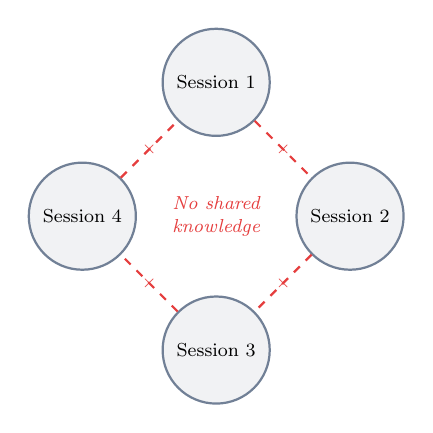
\begin{tikzpicture}[scale=0.85, every node/.style={transform shape}]
  % Sessions as disconnected circles
  \foreach \i/\lbl in {1/Session 1, 2/Session 2, 3/Session 3, 4/Session 4} {
    \pgfmathsetmacro{\ang}{90 - (\i-1)*90}
    \node[circle, draw=cGray, fill=cGray!10, minimum size=1.6cm,
          font=\footnotesize, align=center, line width=0.8pt]
      (s\i) at (\ang:2cm) {\lbl};
  }

  % X marks between them
  \foreach \a/\b in {1/2, 2/3, 3/4, 4/1} {
    \draw[cRed, thick, dashed] (s\a) -- (s\b)
      node[midway, font=\scriptsize\bfseries, text=cRed] {$\times$};
  }

  % Center label
  \node[font=\footnotesize\itshape, text=cRed, align=center] at (0,0)
    {No shared\\knowledge};
\end{tikzpicture}

\end{column}
\end{columns}

\end{frame}

% ══════════════════════════════════════════════════════════════
% THE VISION
% ══════════════════════════════════════════════════════════════
\begin{frame}[shrink=3]{What If Your AI Assistant Could Learn?}

\begin{columns}[T]
\begin{column}{0.48\textwidth}

\begin{exampleblock}{The Goal}
\begin{itemize}
  \item Remember what worked --- and what didn't
  \item Know project conventions without being told
  \item Distinguish project-specific from universal knowledge
  \item Codify repeatable workflows automatically
  \item Catch known errors before they happen
\end{itemize}
\end{exampleblock}

\medskip

\textcolor{cGreen}{\textbf{Key insight:}} Claude Code already has the infrastructure for this. \textbf{You just have to build the architecture.}

\end{column}
\begin{column}{0.48\textwidth}

\centering
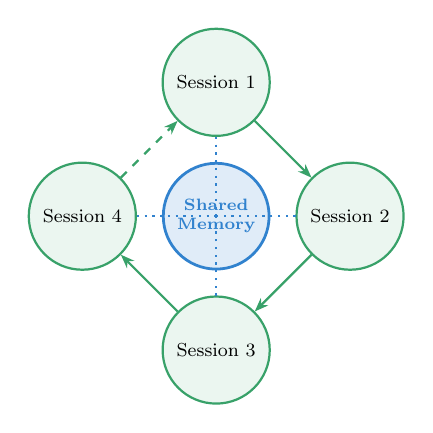
\begin{tikzpicture}[scale=0.85, every node/.style={transform shape}]
  % Sessions as connected circles
  \foreach \i/\lbl in {1/Session 1, 2/Session 2, 3/Session 3, 4/Session 4} {
    \pgfmathsetmacro{\ang}{90 - (\i-1)*90}
    \node[circle, draw=cGreen, fill=cGreen!10, minimum size=1.6cm,
          font=\footnotesize, align=center, line width=0.8pt]
      (s\i) at (\ang:2cm) {\lbl};
  }

  % Connecting arrows
  \foreach \a/\b in {1/2, 2/3, 3/4} {
    \draw[arw=cGreen] (s\a) -- (s\b);
  }
  \draw[arw=cGreen, dashed] (s4) -- (s1);

  % Center hub
  \node[circle, draw=cAccent, fill=cAccent!15, minimum size=1.4cm,
        font=\scriptsize\bfseries, align=center, text=cAccent, line width=1pt]
    at (0,0) {Shared\\Memory};

  % Spokes to hub
  \foreach \i in {1,...,4} {
    \draw[cAccent, thick, dotted] (s\i) -- (0,0);
  }
\end{tikzpicture}

\end{column}
\end{columns}

\end{frame}

% ══════════════════════════════════════════════════════════════
% ARCHITECTURE OVERVIEW
% ══════════════════════════════════════════════════════════════
\begin{frame}{The Three-Layer Architecture}

\centering
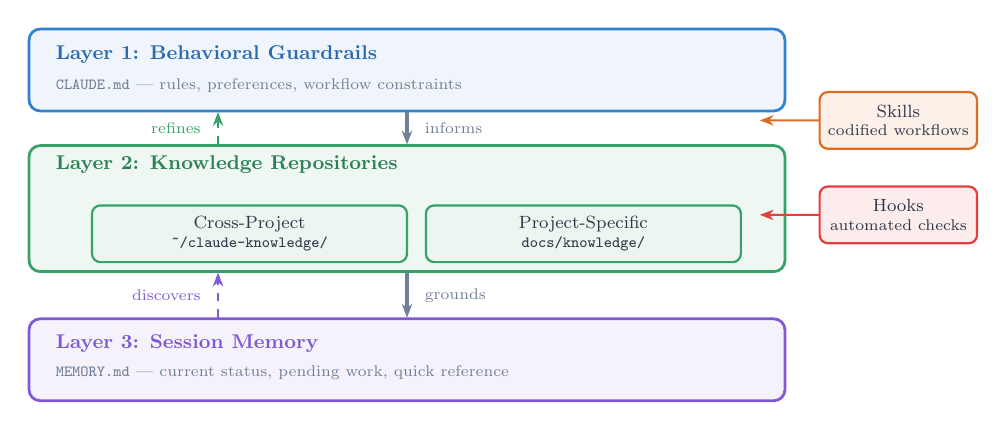
\begin{tikzpicture}[scale=0.8, every node/.style={transform shape}]

  % Layer 3 (bottom) — Session Memory
  \node[layerbox=cPurple, minimum height=1.3cm] (L3) at (0,0) {};
  \node[font=\small\bfseries, text=cPurple, anchor=west] at (-5.7,0.25)
    {Layer 3: Session Memory};
  \node[font=\scriptsize, text=cGray, anchor=west] at (-5.7,-0.2)
    {\texttt{MEMORY.md} --- current status, pending work, quick reference};

  % Layer 2 (middle) — Knowledge Repositories
  \node[layerbox=cGreen, minimum height=2.0cm] (L2) at (0,2.4) {};
  \node[font=\small\bfseries, text=cGreen!80!black, anchor=west] at (-5.7,3.1)
    {Layer 2: Knowledge Repositories};

  % Sub-boxes in Layer 2
  \node[smallbox=cGreen, minimum width=5.0cm] at (-2.5,2.0)
    {Cross-Project\\[-1pt]\scriptsize\texttt{\textasciitilde/claude-knowledge/}};
  \node[smallbox=cGreen, minimum width=5.0cm] at (2.8,2.0)
    {Project-Specific\\[-1pt]\scriptsize\texttt{docs/knowledge/}};

  % Layer 1 (top) — Behavioral Guardrails
  \node[layerbox=cAccent, minimum height=1.3cm] (L1) at (0,4.6) {};
  \node[font=\small\bfseries, text=cAccentDark, anchor=west] at (-5.7,4.85)
    {Layer 1: Behavioral Guardrails};
  \node[font=\scriptsize, text=cGray, anchor=west] at (-5.7,4.35)
    {\texttt{CLAUDE.md} --- rules, preferences, workflow constraints};

  % Active components on the right
  \node[smallbox=cOrange, minimum width=2.5cm] (skills) at (7.8,3.8)
    {Skills\\[-1pt]\scriptsize codified workflows};
  \node[smallbox=cRed, minimum width=2.5cm] (hooks) at (7.8,2.3)
    {Hooks\\[-1pt]\scriptsize automated checks};

  % Arrows from active components
  \draw[arw=cOrange, thick] (skills.west) -- (5.6,3.8);
  \draw[arw=cRed, thick] (hooks.west) -- (5.6,2.3);

  % Vertical flow arrows
  \draw[arw=cGray, line width=1.5pt] (L1.south) -- (L2.north)
    node[midway, right=4pt, font=\scriptsize, text=cGray] {informs};
  \draw[arw=cGray, line width=1.5pt] (L2.south) -- (L3.north)
    node[midway, right=4pt, font=\scriptsize, text=cGray] {grounds};

  % Upward feedback arrow
  \draw[arw=cPurple, dashed, line width=1pt]
    ([xshift=-3cm]L3.north) -- ([xshift=-3cm]L2.south)
    node[midway, left=4pt, font=\scriptsize, text=cPurple] {discovers};
  \draw[arw=cGreen, dashed, line width=1pt]
    ([xshift=-3cm]L2.north) -- ([xshift=-3cm]L1.south)
    node[midway, left=4pt, font=\scriptsize, text=cGreen] {refines};

\end{tikzpicture}

\end{frame}

% ══════════════════════════════════════════════════════════════
% LAYER 1: BEHAVIORAL GUARDRAILS
% ══════════════════════════════════════════════════════════════
\begin{frame}[shrink=8]{Layer 1: Behavioral Guardrails}

\textbf{Two levels of \texttt{CLAUDE.md} files shape every interaction:}

\smallskip

\begin{columns}[T]
\begin{column}{0.47\textwidth}

\begin{block}{Global (\texttt{\textasciitilde/.claude/CLAUDE.md})}
\begin{itemize}\small
  \item Your identity, expertise, communication style
  \item When to ask vs.\ proceed
  \item What frustrates you about AI assistants
  \item Universal rules (verify every step, no silent assumptions)
  \item Pointer to cross-project knowledge
\end{itemize}
\end{block}

\end{column}
\begin{column}{0.47\textwidth}

\begin{block}{Project (\texttt{project/CLAUDE.md})}
\begin{itemize}\small
  \item Key variables and their meanings
  \item Directory structure conventions
  \item ``Read these files first'' instructions
  \item Knowledge management rules
  \item Do-file conventions
\end{itemize}
\end{block}

\end{column}
\end{columns}

\smallskip

\begin{exampleblock}{Why This Matters}
\small Without guardrails, Claude will reorganize code you didn't ask it to touch, add unnecessary error handling, make silent assumptions about methodology, and apologize instead of asking.
With guardrails, it works \textit{the way you work}.
\end{exampleblock}

\end{frame}

% ══════════════════════════════════════════════════════════════
% LAYER 2A: CROSS-PROJECT KNOWLEDGE
% ══════════════════════════════════════════════════════════════
\begin{frame}[shrink=5]{Layer 2a: Cross-Project Knowledge}

\texttt{\textasciitilde/claude-knowledge/} --- a git-tracked repository shared across all projects.

\medskip

\centering
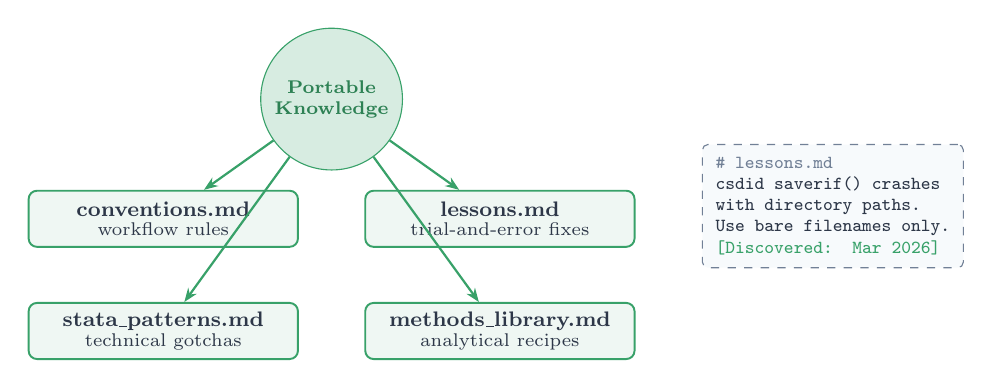
\begin{tikzpicture}[
  fnode/.style={draw=cGreen, fill=cGreen!8, rounded corners=3pt,
    minimum width=3.6cm, minimum height=0.75cm,
    font=\footnotesize, text=cPrimary, line width=0.7pt, align=center},
  scale=0.95, every node/.style={transform shape}
]
  \node[fnode] (conv) at (0,0) {\textbf{conventions.md}\\[-2pt]\scriptsize workflow rules};
  \node[fnode] (les) at (4.5,0) {\textbf{lessons.md}\\[-2pt]\scriptsize trial-and-error fixes};
  \node[fnode] (stat) at (0,-1.5) {\textbf{stata\_patterns.md}\\[-2pt]\scriptsize technical gotchas};
  \node[fnode] (meth) at (4.5,-1.5) {\textbf{methods\_library.md}\\[-2pt]\scriptsize analytical recipes};

  % Hub
  \node[circle, draw=cGreen, fill=cGreen!20, minimum size=1.1cm,
        font=\scriptsize\bfseries, text=cGreen!80!black, align=center]
    (hub) at (2.25,1.6) {Portable\\Knowledge};

  \draw[arw=cGreen] (hub) -- (conv);
  \draw[arw=cGreen] (hub) -- (les);
  \draw[arw=cGreen] (hub) -- (stat);
  \draw[arw=cGreen] (hub) -- (meth);

  % Example annotation
  \node[draw=cGray, dashed, rounded corners=2pt, fill=cCodeBg,
        font=\scriptsize\ttfamily, text=cPrimary, align=left,
        anchor=north west, inner sep=5pt] at (7.2, 1.0) {%
    \textcolor{cGray}{\# lessons.md}\\
    csdid saverif() crashes\\
    with directory paths.\\
    Use bare filenames only.\\
    \textcolor{cGreen}{[Discovered: Mar 2026]}%
  };

\end{tikzpicture}

\bigskip

\begin{columns}[T]
\begin{column}{0.47\textwidth}
\small\textcolor{cGreen}{\textbf{What belongs here:}}
\begin{itemize}\footnotesize
  \item Software bugs and workarounds
  \item Process conventions (verify every step)
  \item Analytical method recipes
\end{itemize}
\end{column}
\begin{column}{0.47\textwidth}
\small\textcolor{cRed}{\textbf{What does NOT belong:}}
\begin{itemize}\footnotesize
  \item Project-specific variable definitions
  \item Regression results or coefficients
  \item Sample construction details
\end{itemize}
\end{column}
\end{columns}

\end{frame}

% ══════════════════════════════════════════════════════════════
% LAYER 2B: PROJECT KNOWLEDGE
% ══════════════════════════════════════════════════════════════
\begin{frame}[shrink=12]{Layer 2b: Project Knowledge Repository}

\texttt{docs/knowledge/} --- single source of truth for everything about \textit{this} project.

\smallskip

\centering
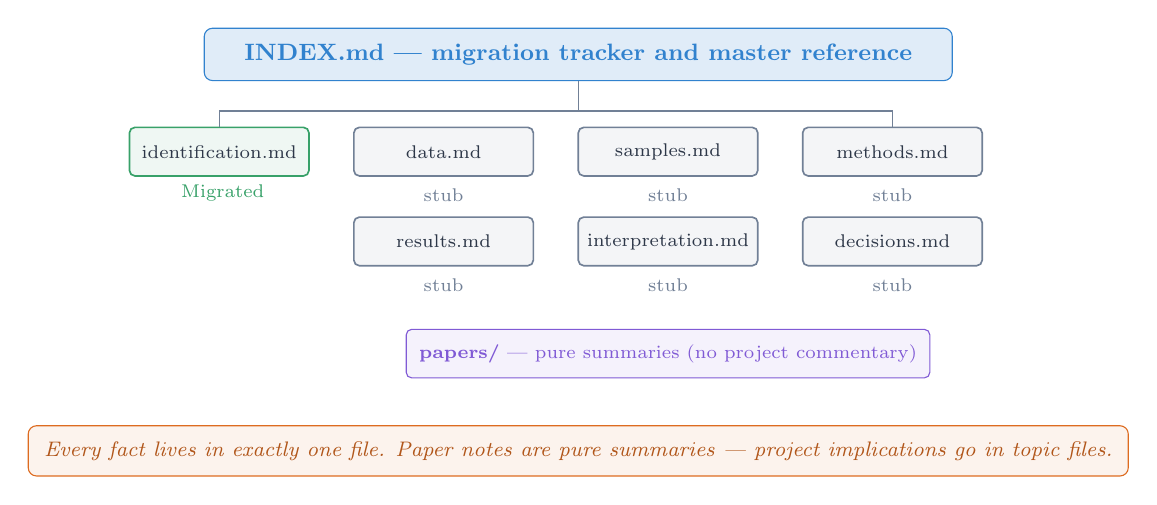
\begin{tikzpicture}[
  tfile/.style={draw=#1, fill=#1!8, rounded corners=2pt,
    minimum width=2.4cm, minimum height=0.65cm,
    font=\scriptsize, text=cPrimary, line width=0.6pt, align=center},
  scale=0.95, every node/.style={transform shape}
]
  % Index at top
  \node[draw=cAccent, fill=cAccent!15, rounded corners=3pt,
        minimum width=10cm, minimum height=0.7cm,
        font=\small\bfseries, text=cAccent] (idx) at (0,2.5)
    {INDEX.md --- migration tracker and master reference};

  % Row 1: Migrated
  \node[tfile=cGreen] (id) at (-4.8,1.2) {identification.md};
  \node[font=\scriptsize, text=cGreen] at (-4.8, 0.65) {\checkmark~Migrated};

  % Row 1: Stubs
  \node[tfile=cGray] (data) at (-1.8,1.2) {data.md};
  \node[tfile=cGray] (samp) at (1.2,1.2) {samples.md};
  \node[tfile=cGray] (meth) at (4.2,1.2) {methods.md};

  \node[tfile=cGray] (res) at (-1.8,0.0) {results.md};
  \node[tfile=cGray] (int) at (1.2,0.0) {interpretation.md};
  \node[tfile=cGray] (dec) at (4.2,0.0) {decisions.md};

  % Stub labels
  \foreach \n in {data, samp, meth, res, int, dec} {
    \node[font=\scriptsize, text=cGray] at (\n.south) [below=1pt] {stub};
  }

  % Papers subdir
  \node[draw=cPurple, fill=cPurple!8, rounded corners=2pt,
        minimum width=7cm, minimum height=0.65cm,
        font=\scriptsize, text=cPurple] (pap) at (1.2,-1.5)
    {\textbf{papers/} --- pure summaries (no project commentary)};

  % Arrows from index
  \draw[cGray, thin] (idx.south) -- ++(0,-0.4) -| (id.north);
  \draw[cGray, thin] (idx.south) -- ++(0,-0.4) -| (meth.north);

  % Key principle
  \node[draw=cOrange, fill=cOrange!8, rounded corners=3pt,
        font=\footnotesize\itshape, text=cOrange!80!black,
        inner sep=6pt, align=center] at (0,-2.8)
    {Every fact lives in exactly one file.
     Paper notes are pure summaries --- project implications go in topic files.};

\end{tikzpicture}

\end{frame}

% ══════════════════════════════════════════════════════════════
% LAYER 3: SESSION MEMORY
% ══════════════════════════════════════════════════════════════
\begin{frame}{Layer 3: Session Memory}

\texttt{MEMORY.md} --- auto-loaded every session, carries forward across conversations.

\bigskip

\begin{columns}[T]
\begin{column}{0.47\textwidth}

\begin{block}{Persistent (stable across sessions)}
\begin{itemize}\small
  \item Authors, collaborators
  \item File paths, software locations
  \item Key variable names and definitions
  \item User preferences and workflow rules
\end{itemize}
\end{block}

\end{column}
\begin{column}{0.47\textwidth}

\begin{alertblock}{Ephemeral (verify at session start)}
\begin{itemize}\small
  \item Current project status
  \item Pending work items
  \item Last compilation dates
  \item Recently completed tasks
\end{itemize}
\end{alertblock}

\end{column}
\end{columns}

\bigskip

\begin{exampleblock}{Design Principle}
Separate what \textit{persists} from what \textit{decays}. Ephemeral sections are date-stamped and labeled ``verify at session start'' so new sessions know what might be stale.
\end{exampleblock}

\end{frame}

% ══════════════════════════════════════════════════════════════
% THE KNOWLEDGE LIFECYCLE
% ══════════════════════════════════════════════════════════════
\begin{frame}{The Knowledge Lifecycle}

\centering
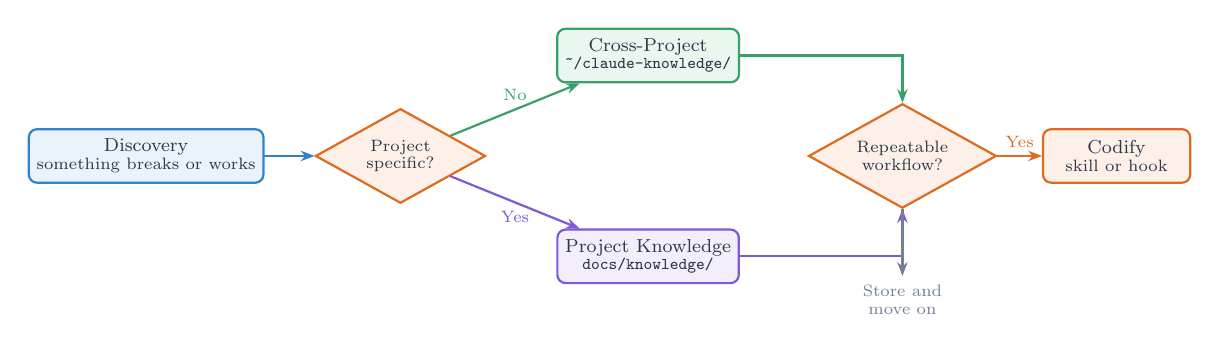
\begin{tikzpicture}[scale=0.85, every node/.style={transform shape}]

  % Nodes in a flow
  \node[flownode, minimum width=2.4cm] (disc) at (0,0) {Discovery\\[-2pt]\scriptsize something breaks or works};

  \node[decisionnode] (q1) at (3.8,0) {\scriptsize Project\\[-2pt]\scriptsize specific?};

  \node[flownode, fill=cGreen!10, draw=cGreen, minimum width=2.6cm]
    (cross) at (7.5,1.5) {Cross-Project\\[-2pt]\scriptsize\texttt{\textasciitilde/claude-knowledge/}};

  \node[flownode, fill=cPurple!10, draw=cPurple, minimum width=2.6cm]
    (proj) at (7.5,-1.5) {Project Knowledge\\[-2pt]\scriptsize\texttt{docs/knowledge/}};

  \node[decisionnode] (q2) at (11.3,0) {\scriptsize Repeatable\\[-2pt]\scriptsize workflow?};

  \node[flownode, fill=cOrange!10, draw=cOrange, minimum width=2.2cm]
    (skill) at (14.5,0) {Codify\\[-2pt]\scriptsize skill or hook};

  % Arrows
  \draw[arw] (disc) -- (q1);
  \draw[arw=cGreen] (q1) -- node[above, font=\scriptsize, text=cGreen] {No} (cross);
  \draw[arw=cPurple] (q1) -- node[below, font=\scriptsize, text=cPurple] {Yes} (proj);
  \draw[arw=cGreen] (cross) -| (q2);
  \draw[arw=cPurple] (proj) -| (q2);
  \draw[arw=cOrange] (q2) -- node[above, font=\scriptsize, text=cOrange] {Yes} (skill);

  % No path from q2
  \draw[arw=cGray] (q2.south) -- ++(0,-1.0)
    node[below, font=\scriptsize, text=cGray, align=center] {Store and\\move on};

\end{tikzpicture}

\bigskip

\begin{columns}[T]
\begin{column}{0.47\textwidth}
\small\textbf{Retain the fix, forget the failures.}\\[3pt]
\footnotesize After 12 failed approaches and 1 solution, only the solution enters the knowledge base --- with enough context to prevent the same failure mode.
\end{column}
\begin{column}{0.47\textwidth}
\small\textbf{One fact, one file.}\\[3pt]
\footnotesize When knowledge is discovered or corrected, update the canonical source immediately. No duplication across files.
\end{column}
\end{columns}

\end{frame}

% ══════════════════════════════════════════════════════════════
% SKILLS: CODIFIED WORKFLOWS
% ══════════════════════════════════════════════════════════════
\begin{frame}{Skills: Codified Workflows}

Skills are reusable, multi-step procedures invoked with \texttt{/skill-name}.

\bigskip

\centering
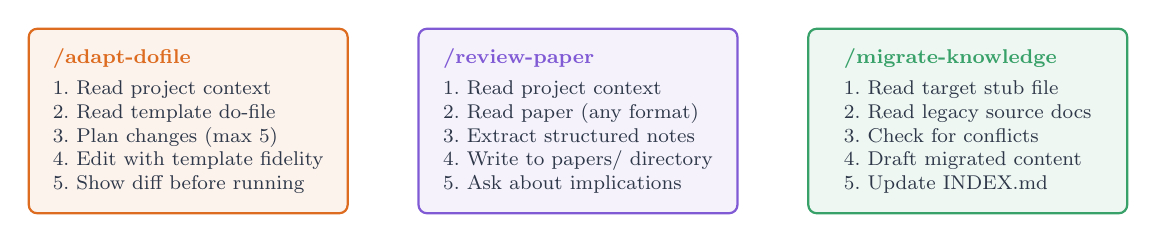
\begin{tikzpicture}[
  sbox/.style={draw=#1, fill=#1!8, rounded corners=3pt,
    minimum width=4.5cm, minimum height=2.2cm,
    font=\footnotesize, text=cPrimary, line width=0.8pt, align=left,
    inner sep=8pt},
  scale=0.9, every node/.style={transform shape}
]

  \node[sbox=cOrange] (s1) at (0,0) {%
    \textcolor{cOrange}{\textbf{/adapt-dofile}}\\[3pt]
    1.~Read project context\\
    2.~Read template do-file\\
    3.~Plan changes (max 5)\\
    4.~Edit with template fidelity\\
    5.~Show diff before running%
  };

  \node[sbox=cPurple] (s2) at (5.5,0) {%
    \textcolor{cPurple}{\textbf{/review-paper}}\\[3pt]
    1.~Read project context\\
    2.~Read paper (any format)\\
    3.~Extract structured notes\\
    4.~Write to papers/ directory\\
    5.~Ask about implications%
  };

  \node[sbox=cGreen] (s3) at (11,0) {%
    \textcolor{cGreen}{\textbf{/migrate-knowledge}}\\[3pt]
    1.~Read target stub file\\
    2.~Read legacy source docs\\
    3.~Check for conflicts\\
    4.~Draft migrated content\\
    5.~Update INDEX.md%
  };

\end{tikzpicture}

\smallskip

\begin{block}{What Makes a Good Skill}
\begin{itemize}\footnotesize
  \item A workflow you've done 3+ times with the same structure
  \item A ``read these files first'' preamble that gets repeated
  \item A communication product that follows a consistent template
  \item Clear inputs (arguments), clear outputs (files), clear constraints (rules)
\end{itemize}
\end{block}

\end{frame}

% ══════════════════════════════════════════════════════════════
% HOOKS: AUTOMATED VALIDATION
% ══════════════════════════════════════════════════════════════
\begin{frame}[shrink=10]{Hooks: Automated Validation}

\small Hooks fire before or after tool use --- they enforce rules without requiring manual attention.

\smallskip

\begin{columns}[T]
\begin{column}{0.47\textwidth}

\begin{block}{PreToolUse: Large File Guard}
\small
Fires before \texttt{Read}. If a file exceeds 500KB, warns Claude to use \texttt{offset/limit} or convert to text first.
\medskip

\textit{Prevents}: accidentally dumping huge datasets into context, wasting the context window.
\end{block}

\end{column}
\begin{column}{0.47\textwidth}

\begin{block}{PostToolUse: Stata Log Validator}
\small
Fires after \texttt{Bash} when the command contains \texttt{stata-mp}. Scans output for:
\begin{itemize}\footnotesize
  \item \texttt{r(...)} error codes
  \item ``no observations'' warnings
  \item Memory allocation failures
  \item ``variable not found'' errors
\end{itemize}
\medskip

\textit{Prevents}: silently continuing past Stata errors.
\end{block}

\end{column}
\end{columns}

\smallskip

\begin{exampleblock}{When to Create a Hook}
\small When a manual check is repeated after every run, or an error pattern has been caught and fixed more than once. Hooks belong at the \textit{global} level (\texttt{\textasciitilde/.claude/settings.json}) if they apply across projects.
\end{exampleblock}

\end{frame}

% ══════════════════════════════════════════════════════════════
% SINGLE SOURCE OF TRUTH
% ══════════════════════════════════════════════════════════════
\begin{frame}{The ``Single Source of Truth'' Principle}

\centering
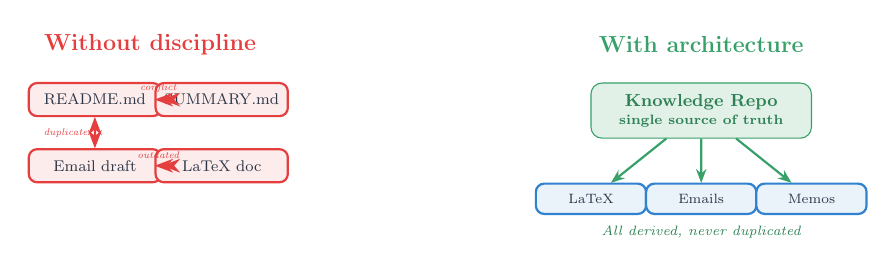
\begin{tikzpicture}[scale=0.7, every node/.style={transform shape}]

  % BAD side
  \node[font=\large\bfseries, text=cRed] at (-5.5, 3.0) {Without discipline};

  \node[smallbox=cRed, minimum width=2.4cm, minimum height=0.6cm]
    (b1) at (-6.5, 2.0) {README.md};
  \node[smallbox=cRed, minimum width=2.4cm, minimum height=0.6cm]
    (b2) at (-4.2, 2.0) {SUMMARY.md};
  \node[smallbox=cRed, minimum width=2.4cm, minimum height=0.6cm]
    (b3) at (-6.5, 0.8) {Email draft};
  \node[smallbox=cRed, minimum width=2.4cm, minimum height=0.6cm]
    (b4) at (-4.2, 0.8) {LaTeX doc};

  % Contradictions
  \draw[cRed, thick, {Stealth}-{Stealth}] (b1) -- (b2)
    node[midway, above, font=\tiny\itshape, text=cRed] {conflict};
  \draw[cRed, thick, {Stealth}-{Stealth}] (b3) -- (b4)
    node[midway, above, font=\tiny\itshape, text=cRed] {outdated};
  \draw[cRed, thick, {Stealth}-{Stealth}] (b1) -- (b3)
    node[midway, left, font=\tiny\itshape, text=cRed] {duplicate};

  % GOOD side
  \node[font=\large\bfseries, text=cGreen] at (4.5, 3.0) {With architecture};

  % Canonical source
  \node[draw=cGreen, fill=cGreen!15, rounded corners=4pt,
        minimum width=4cm, minimum height=1cm,
        font=\small\bfseries, text=cGreen!80!black, align=center]
    (canon) at (4.5, 1.8) {Knowledge Repo\\[-2pt]\scriptsize single source of truth};

  % Derived products
  \node[smallbox=cAccent, minimum width=2.0cm, minimum height=0.55cm]
    (d1) at (2.5, 0.2) {\scriptsize LaTeX};
  \node[smallbox=cAccent, minimum width=2.0cm, minimum height=0.55cm]
    (d2) at (4.5, 0.2) {\scriptsize Emails};
  \node[smallbox=cAccent, minimum width=2.0cm, minimum height=0.55cm]
    (d3) at (6.5, 0.2) {\scriptsize Memos};

  \draw[arw=cGreen] (canon) -- (d1);
  \draw[arw=cGreen] (canon) -- (d2);
  \draw[arw=cGreen] (canon) -- (d3);

  \node[font=\scriptsize\itshape, text=cGreen!80!black] at (4.5, -0.4)
    {All derived, never duplicated};

\end{tikzpicture}

\smallskip

\begin{alertblock}{The Rule}
\small When a fact changes, you update \textbf{one file}. Everything downstream regenerates from it. If you find the same fact in two places, you have a bug in your architecture.
\end{alertblock}

\end{frame}

% ══════════════════════════════════════════════════════════════
% LESSONS LEARNED LOOP
% ══════════════════════════════════════════════════════════════
\begin{frame}{The Lessons Learned Loop}

\centering
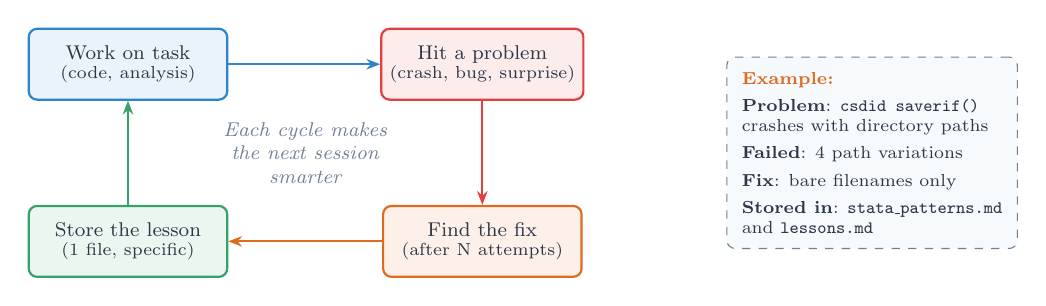
\begin{tikzpicture}[scale=0.9, every node/.style={transform shape}]

  % Cycle nodes
  \node[flownode, minimum width=2.8cm, minimum height=1cm]
    (work) at (0,2.5) {Work on task\\[-2pt]\scriptsize (code, analysis)};

  \node[flownode, fill=cRed!10, draw=cRed, minimum width=2.8cm, minimum height=1cm]
    (fail) at (5,2.5) {Hit a problem\\[-2pt]\scriptsize (crash, bug, surprise)};

  \node[flownode, fill=cOrange!10, draw=cOrange, minimum width=2.8cm, minimum height=1cm]
    (fix) at (5,0) {Find the fix\\[-2pt]\scriptsize (after N attempts)};

  \node[flownode, fill=cGreen!10, draw=cGreen, minimum width=2.8cm, minimum height=1cm]
    (store) at (0,0) {Store the lesson\\[-2pt]\scriptsize (1 file, specific)};

  % Cycle arrows
  \draw[arw] (work) -- (fail);
  \draw[arw=cRed] (fail) -- (fix);
  \draw[arw=cOrange] (fix) -- (store);
  \draw[arw=cGreen] (store) -- (work);

  % Center annotation
  \node[font=\footnotesize\itshape, text=cGray, align=center] at (2.5,1.25)
    {Each cycle makes\\the next session\\smarter};

  % Example callout
  \node[draw=cGray, dashed, rounded corners=3pt, fill=cCodeBg,
        font=\scriptsize, text=cPrimary, align=left,
        inner sep=6pt] at (10.5, 1.25) {%
    \textcolor{cOrange}{\textbf{Example:}}\\[3pt]
    \textbf{Problem}: \texttt{csdid saverif()}\\
    crashes with directory paths\\[3pt]
    \textbf{Failed}: 4 path variations\\[3pt]
    \textbf{Fix}: bare filenames only\\[3pt]
    \textbf{Stored in}: \texttt{stata\_patterns.md}\\
    and \texttt{lessons.md}%
  };

\end{tikzpicture}

\bigskip

\small The key discipline: after debugging, \textbf{immediately} distill the lesson into the knowledge base. Don't promise to do it later. The 12 failed attempts get discarded; the fix gets preserved with just enough context to prevent the same failure.

\end{frame}

% ══════════════════════════════════════════════════════════════
% WHAT CHANGES VS WHAT PERSISTS
% ══════════════════════════════════════════════════════════════
\begin{frame}[shrink=15]{Inter-Project vs.\ Intra-Project Knowledge}

\centering
\small
\renewcommand{\arraystretch}{1.25}
\begin{tabular}{>{\raggedright}p{3.0cm} >{\raggedright}p{4.5cm} >{\raggedright\arraybackslash}p{4.5cm}}
  \toprule
  & \textcolor{cGreen}{\textbf{Cross-Project}} & \textcolor{cPurple}{\textbf{Project-Specific}} \\
  & \scriptsize\texttt{\textasciitilde/claude-knowledge/} & \scriptsize\texttt{docs/knowledge/} \\
  \midrule
  \textbf{Content} &
    Software gotchas, process conventions, analytical recipes, debugging lessons &
    Variable definitions, sample construction, regression results, identification strategy \\
  \textbf{Lifespan} &
    Indefinite --- survives project completion &
    Tied to project lifecycle \\
  \textbf{Audience} &
    Any future project's Claude instance &
    Only this project's Claude instance \\
  \textbf{Example} &
    ``\texttt{csdid} crashes on >2.5M obs'' &
    ``Panel A uses oversample only due to memory constraints'' \\
  \textbf{Update trigger} &
    New software discovery or workflow refinement &
    New results, methodology change, or course correction \\
  \bottomrule
\end{tabular}

\bigskip

\begin{block}{The Test}
\small If you started a completely different research project tomorrow, would this knowledge still be useful? \textcolor{cGreen}{\textbf{Yes}} $\rightarrow$ cross-project. \textcolor{cPurple}{\textbf{No}} $\rightarrow$ project-specific.
\end{block}

\end{frame}

% ══════════════════════════════════════════════════════════════
% BUILDING YOUR OWN: STEP 1
% ══════════════════════════════════════════════════════════════
\begin{frame}{Building Your Own: Step 1 --- Global Configuration}

\begin{exampleblock}{Time: 30 minutes. Impact: every future session.}
\end{exampleblock}

\begin{enumerate}\small
  \item \textbf{Create \texttt{\textasciitilde/.claude/CLAUDE.md}} --- your global instruction file.
    \begin{itemize}\footnotesize
      \item Who you are, your expertise level, communication preferences
      \item Your frustrations with AI assistants (be specific!)
      \item When Claude should ask vs.\ proceed autonomously
      \item Universal rules (``verify every step,'' ``no silent assumptions'')
    \end{itemize}

  \item \textbf{Create \texttt{\textasciitilde/claude-knowledge/}} --- your cross-project knowledge repo.
    \begin{itemize}\footnotesize
      \item \texttt{conventions.md} --- process rules that apply everywhere
      \item \texttt{lessons.md} --- debugging insights (start empty, grows organically)
      \item One file per software/tool you use heavily (e.g., \texttt{stata\_patterns.md})
      \item Initialize as a git repo for version tracking
    \end{itemize}

  \item \textbf{Configure \texttt{\textasciitilde/.claude/settings.json}} --- permissions and hooks.
    \begin{itemize}\footnotesize
      \item Set \texttt{additionalDirectories} to include your knowledge repo
      \item Add a PreToolUse hook for large file warnings
    \end{itemize}
\end{enumerate}

\end{frame}

% ══════════════════════════════════════════════════════════════
% BUILDING YOUR OWN: STEP 2
% ══════════════════════════════════════════════════════════════
\begin{frame}[shrink=5]{Building Your Own: Step 2 --- Project Knowledge}

\begin{exampleblock}{Time: 1 hour per project. Impact: eliminates re-teaching.}
\end{exampleblock}

\begin{enumerate}\small
  \item \textbf{Create \texttt{project/CLAUDE.md}} --- project-specific instructions.
    \begin{itemize}\footnotesize
      \item ``Read these files before doing anything''
      \item Key variables, directory structure, naming conventions
      \item Pointer to the knowledge repo
    \end{itemize}

  \item \textbf{Create \texttt{docs/knowledge/}} with an \texttt{INDEX.md} and topic files.
    \begin{itemize}\footnotesize
      \item Start with stubs --- list what each file \textit{will} contain
      \item Migrate incrementally as you work (don't try to do it all at once)
      \item One fully-written file is better than eight half-written ones
    \end{itemize}

  \item \textbf{Set up \texttt{MEMORY.md}} in your project memory directory.
    \begin{itemize}\footnotesize
      \item Persistent section: authors, paths, key variables, preferences
      \item Ephemeral section: current status, pending work (date-stamped)
      \item Keep it under 200 lines (it's loaded into every context window)
    \end{itemize}
\end{enumerate}

\medskip

\begin{alertblock}{Common Mistake}
\small Don't try to document everything upfront. Start working, and when Claude asks a question you've answered before, \textit{that's} what goes in the knowledge repo.
\end{alertblock}

\end{frame}

% ══════════════════════════════════════════════════════════════
% BUILDING YOUR OWN: STEP 3
% ══════════════════════════════════════════════════════════════
\begin{frame}[shrink=10]{Building Your Own: Step 3 --- Skills and Hooks}

\begin{exampleblock}{Time: ongoing. Impact: compounds over time.}
\end{exampleblock}

\smallskip

\begin{block}{When to Create a Skill}
\small A skill is a multi-step workflow saved as a \texttt{SKILL.md} file in \texttt{.claude/skills/}.
\begin{itemize}\footnotesize
  \item You've done the same workflow 3+ times
  \item It has a ``read these files first'' preamble
  \item It produces a consistent output format (paper notes, adapted code, migrated docs)
  \item It has clear rules that prevent Claude from over-engineering
\end{itemize}
\end{block}

\begin{block}{When to Create a Hook}
\small A hook is a shell command that fires before/after a tool in \texttt{settings.json}.
\begin{itemize}\footnotesize
  \item A manual check is repeated after every execution
  \item An error pattern has burned you more than once
  \item A safety guard needs to be enforced without thinking about it
\end{itemize}
\end{block}

\medskip

\small\textbf{Skill anatomy:} Name, description, arguments, 3--5 steps, rules.\\
\textbf{Hook anatomy:} Trigger (Pre/PostToolUse), matcher (tool name), shell command.

\end{frame}

% ══════════════════════════════════════════════════════════════
% KEY PRINCIPLES
% ══════════════════════════════════════════════════════════════
\begin{frame}{Key Principles}

\centering
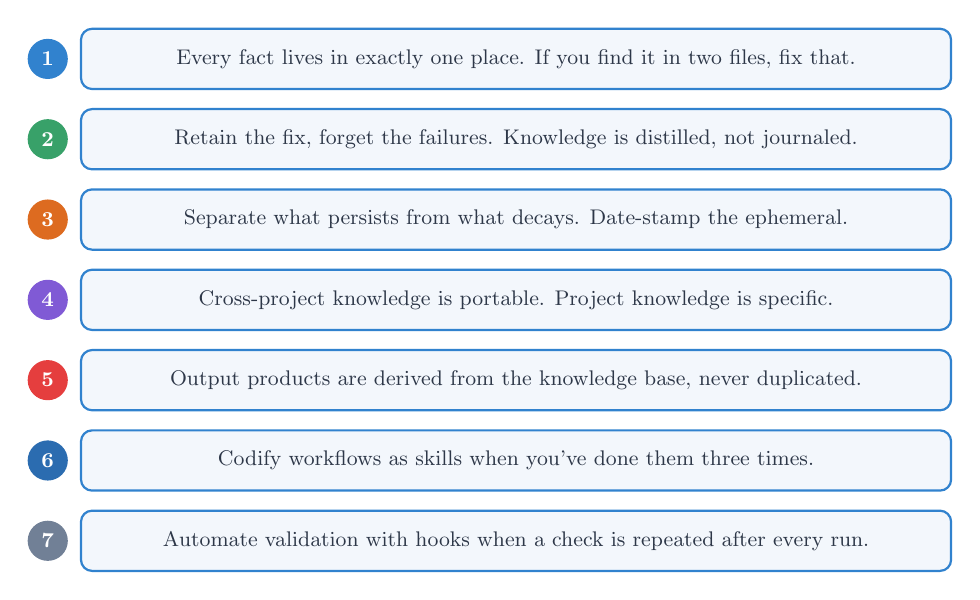
\begin{tikzpicture}[
  pbox/.style={draw=cAccent, fill=cAccent!6, rounded corners=4pt,
    minimum width=13cm, minimum height=0.9cm,
    font=\small, text=cPrimary, line width=0.8pt, align=left,
    inner xsep=10pt},
  num/.style={circle, fill=#1, text=white, font=\small\bfseries,
    minimum size=0.6cm, inner sep=0pt},
  scale=0.85, every node/.style={transform shape}
]

  \node[pbox] (p1) at (0, 4.0) {Every fact lives in exactly one place. If you find it in two files, fix that.};
  \node[num=cAccent, left=5pt] at (p1.west) {1};

  \node[pbox] (p2) at (0, 2.8) {Retain the fix, forget the failures. Knowledge is distilled, not journaled.};
  \node[num=cGreen, left=5pt] at (p2.west) {2};

  \node[pbox] (p3) at (0, 1.6) {Separate what persists from what decays. Date-stamp the ephemeral.};
  \node[num=cOrange, left=5pt] at (p3.west) {3};

  \node[pbox] (p4) at (0, 0.4) {Cross-project knowledge is portable. Project knowledge is specific.};
  \node[num=cPurple, left=5pt] at (p4.west) {4};

  \node[pbox] (p5) at (0, -0.8) {Output products are derived from the knowledge base, never duplicated.};
  \node[num=cRed, left=5pt] at (p5.west) {5};

  \node[pbox] (p6) at (0, -2.0) {Codify workflows as skills when you've done them three times.};
  \node[num=cAccentDark, left=5pt] at (p6.west) {6};

  \node[pbox] (p7) at (0, -3.2) {Automate validation with hooks when a check is repeated after every run.};
  \node[num=cGray, left=5pt] at (p7.west) {7};

\end{tikzpicture}

\end{frame}

% ══════════════════════════════════════════════════════════════
% GETTING STARTED CHECKLIST
% ══════════════════════════════════════════════════════════════
\begin{frame}[shrink=15]{Getting Started Checklist}

\renewcommand{\arraystretch}{1.2}
\small
\begin{tabular}{@{}c l l@{}}
  \toprule
  & \textbf{Action} & \textbf{Location} \\
  \midrule
  $\square$ & Write your global instruction file & \texttt{\textasciitilde/.claude/CLAUDE.md} \\
  $\square$ & Create cross-project knowledge repo & \texttt{\textasciitilde/claude-knowledge/} \\
  $\square$ & Add \texttt{conventions.md} with your process rules & \texttt{\textasciitilde/claude-knowledge/} \\
  $\square$ & Add \texttt{lessons.md} (start empty) & \texttt{\textasciitilde/claude-knowledge/} \\
  $\square$ & Configure permissions and directories & \texttt{\textasciitilde/.claude/settings.json} \\
  $\square$ & Add large-file warning hook & \texttt{\textasciitilde/.claude/settings.json} \\
  \midrule
  $\square$ & Write project-level \texttt{CLAUDE.md} & \texttt{project/CLAUDE.md} \\
  $\square$ & Create \texttt{docs/knowledge/INDEX.md} with topic stubs & \texttt{project/docs/knowledge/} \\
  $\square$ & Set up \texttt{MEMORY.md} (persistent + ephemeral) & \texttt{\textasciitilde/.claude/projects/.../memory/} \\
  $\square$ & Fully migrate your most important topic file first & \texttt{project/docs/knowledge/} \\
  \midrule
  $\square$ & Create your first skill after 3 repeated workflows & \texttt{project/.claude/skills/} \\
  $\square$ & Add a validation hook after 2 repeated error checks & \texttt{\textasciitilde/.claude/settings.json} \\
  \bottomrule
\end{tabular}

\bigskip

\begin{exampleblock}{}
\centering\small
Start small. Let the architecture grow from actual pain points, not hypothetical ones.
\end{exampleblock}

\end{frame}

% ══════════════════════════════════════════════════════════════
% CLOSING
% ══════════════════════════════════════════════════════════════
\begin{frame}{}

\centering
\vfill

{\Large\bfseries\textcolor{cPrimary}{The best AI assistant isn't the smartest one.}}

\bigskip

{\Large\textcolor{cAccent}{It's the one that remembers.}}

\vfill

\small\textcolor{cGray}{Built iteratively with Claude Code --- one lesson at a time.}

\vfill

\end{frame}

\end{document}
